\documentclass[border=6pt]{standalone}
\usepackage[T1]{fontenc}\usepackage{lmodern}\usepackage{amsmath,amssymb}\usepackage{xcolor}\usepackage{tikz}
\usetikzlibrary{arrows.meta,positioning,calc,fit,shapes.misc}
% TikZ styles
\tikzset{
  blk/.style={draw, rounded corners=2pt, align=center, font=\small, minimum height=8mm, inner sep=4pt, fill=#1},
  blk/.default=white,
  arr/.style={-{Stealth[length=2.2mm]}, thick},
}
\definecolor{base}{HTML}{FBE3E3}
\definecolor{prop}{HTML}{DDEBFA}
\definecolor{same}{HTML}{EDEDED}
\definecolor{done}{HTML}{DFF1DF}
\definecolor{todo}{HTML}{FFF2CC}

\begin{document}
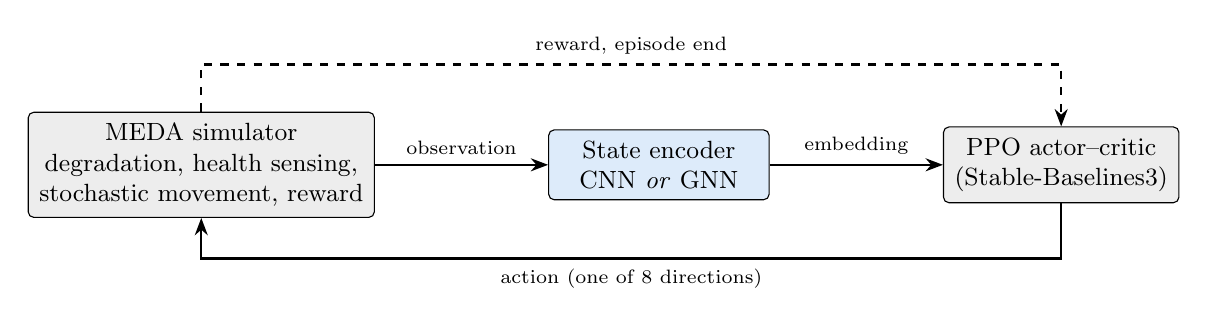
\begin{tikzpicture}[node distance=5mm and 22mm]
  \node[blk=same, minimum width=3.4cm] (sim) {MEDA simulator\\degradation, health sensing,\\stochastic movement, reward};
  \node[blk=prop, right=of sim, minimum width=2.8cm] (enc) {State encoder\\CNN \emph{or} GNN};
  \node[blk=same, right=of enc, minimum width=2.8cm] (ppo) {PPO actor--critic\\(Stable-Baselines3)};
  \draw[arr] (sim) -- node[above, font=\scriptsize]{observation} (enc);
  \draw[arr] (enc) -- node[above, font=\scriptsize]{embedding} (ppo);
  \draw[arr] (ppo.south) -- ++(0,-0.7) -| node[pos=0.25, below, font=\scriptsize]{action (one of 8 directions)} (sim.south);
  \draw[arr, dashed] (sim.north) -- ++(0,0.6) -| node[pos=0.25, above, font=\scriptsize]{reward, episode end} (ppo.north);
\end{tikzpicture}
\end{document}
